\documentclass[12pt]{article}
\usepackage[a4paper, total={7.5in, 11in}]{geometry}
%\usepackage{array}
\usepackage{graphicx, subfig, wrapfig, fancyhdr, lastpage, multicol ,color,arydshln,makecell}
\newcommand\headerMe[2]{\noindent{}#1\hfill#2}
\usepackage[mathscr]{euscript}
\usepackage{tabularray}

\setlength{\columnseprule}{1pt}
\def\columnseprulecolor{\color{blue}}


\pagestyle{fancy}
\fancyhf{}

\cfoot{ \vspace{-0.8cm}\em{Page \thepage \hspace{1pt} / \pageref{LastPage}}}
\begin{document}

\headerMe{Royaume du Maroc}{année scolaire \emph{2024-2025}}\\
\headerMe{Ministère de l'Éducation nationale, }{  Professeur :\emph{Zakaria Haouzan}}\\
\headerMe{du Préscolaire et des Sports}{Établissement : \emph{Lycée SKHOR qualifiant}}\\
\vspace{-1cm}
\begin{center}
Devoir Surveillé  N°1 \\
    2ème année baccalauréat Sciences physiques \\
Durée 2h00
\\
    \vspace{.2cm}
\hrulefill
\Large{Chimie 7pts - 55min}
\hrulefill\\

    %\emph{Les deux parties sont indépendantes}
\end{center}
%end Headerss------------------------
%__________________Chimie ______________________-
%%%%%%%+_+_+_+_+_+_+_+_+_Partie1
\vspace{-1.1cm}
 \section*{Exercice 1 : Suivi temporel d’une transformation chimique \dotfill(7pts) }
 \begin{wrapfigure}[11]{r}{0.50\textwidth}

\begin{center}
	\vspace{-1,2cm}
  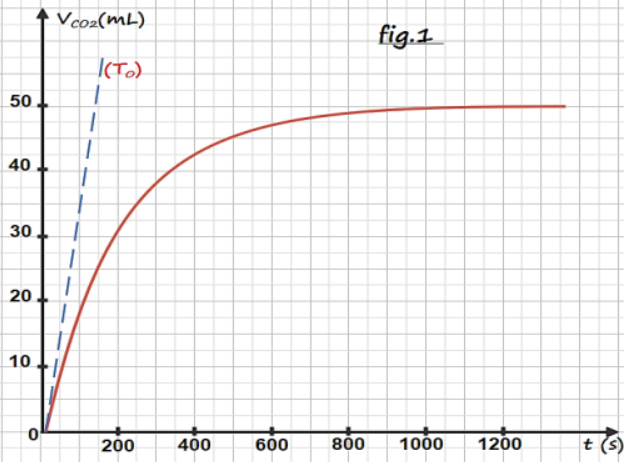
\includegraphics[width=0.50\textwidth ]{./img/fig00.png}
\end{center}
\end{wrapfigure}

L’acide chlorhydrique HCl a plusieurs utilisations tels que : l’élimination de 
dépôts de calcaire dans divers appareils et dans les conduites d’eau. Le calcaire, 
principalement constitué de carbonate de calcium $CaCO_3$, réagit avec une 
solution d’acide chlorhydrique selon l’équation:
$${CaCO_3}_{(s)} + 2H_3O^+_{(aq)} \rightarrow Ca^{2+}_{(aq)} + {CO_2}_{(g)} + 3H_2O_{(l)}$$

Le but de cet exercice est d’étudier la cinétique chimique de cette
réaction en utilisant deux méthodes différentes.
\vspace{-0.7cm}
 \section*{Partie 1 : la Mesure du Volume V($CO_2$)}
\hrulefill
On verse dans un ballon, un volume $V_s = 100mL$ d’une solution d’acide
chlorhydrique $(H_3O_{(aq)}+; Cl^-_{(aq)})$ de concentration $C_1 = 2.10^{-2} mol/L$

A la date $t = 0$, on introduit rapidement dans le ballon, la masse
$m = 0, 300g$ de carbonate de calcium $CaCO_3$ puis on déclenche le

Chronomètre. Le dioxyde de carbone formé est recueilli dans une
éprouvette graduée, à chaque minute, on note le volume $V_{(CO_2)}$ dégagé.


\begin{tabular}{c|l}
	1  & \makecell[l]{ \textbf{1. }Calculer les quantités de matière initiales des réactifs. }\\


	0,5  & \makecell[l]{ \textbf{2. }Dresser le tableau d’avancement de la réaction. }\\


	1  & \makecell[l]{ \textbf{3. } Déterminer l’avancement maximal $x_{max}$ et le réactif limitant.}\\
	
	0,5  & \makecell[l]{ \textbf{4. } Montrer, dans le système d’unités international, que le volume $V_{(CO_2)}$ et l’avancement de la \\réaction $x(t)$ , dans les conditions
	de l’expérience, sont liés \\par la relation : $V_{(CO_2)} = 2,44.10^{-2}.x(t)$}\\

\end{tabular}
Le graphe de la figure 1, ci-dessus, représente la variation du
volume $V_{CO_2}$ de dioxyde de carbone dégagé en fonction du temps, ainsi que la tangente $T_0$ à la date $t = 0$ .

\begin{tabular}{c|l}
	0,75  & \makecell[l]{ \textbf{5. }montrer que : $V_{CO_2} (t_{1/2}) = 25mL$ . En déduire le temps de la demi-réaction $t_{1/2}$. }\\ 

	0,5 & \makecell[l]{ \textbf{6. }Déterminer, dans le système d’unités international, $v(t = 0)$,
la vitesse volumique de la \\réaction à l’instant de date $t = 0$ }\\
	
	0,5    & \makecell[l]{ \textbf{7. }On refait la même expérience précédente à la température
$\theta' = 35$°C. La valeur du temps de \\demi- réaction est-elle
identique, inférieure ou supérieure à la valeur précédente ?
 }\\
\end{tabular}
\begin{center}
	
\begin{center}
\begin{itemize}
	\item 	la température et la pression du gaz constantes : $T = 25^{\circ}C= 298K$ et $P = 1,013.10^{5}Pa$. 
	La masse molaire de $CaCO_3$ est $M = 100g/mol$ et $R =8,31 SI$

\end{itemize}

\end{center}
\end{center}

\vspace{-1cm}
 \section*{Partie 2 : Mesure de conductivité}
L’évolution de la réaction précédente peut être suivie en mesurant
la conductivité $\sigma$ du mélange réactionnel à des instants différents.
On observe expérimentalement une diminution de la conductivité
du mélange réactionnel au cours de la réaction.

\begin{center}
\textbf{\underline{ Données : } }
-  Les conductivités molaire ioniques : 

		$\lambda_{H_3O^+}=35 mS.m^2.mol^{-1}$ ; $ \lambda_{Ca^{2+}}=12mS.m^2.mol^{-1}$ ; $\lambda_{Cl^-}=7,63 mS.m^2.mol^{-1}$

\end{center}

\begin{tabular}{c|l}
	0,75  & \makecell[l]{ \textbf{1. }Calculer $\sigma_i$ la conductivité du mélange réactionnel à l’état initial. }\\


	0,5  & \makecell[l]{ \textbf{2. }Montrer que l’avancement $x(t)$ et $\sigma(t)$ sont liés
	par la relation : $\sigma(t) = -580.x(t) + \sigma_i$ }\\

	
	1  & \makecell[l]{ \textbf{3. }Montrer que la vitesse volumique $v(t)$ de la réaction à l’instant t
	s’écrit sous la forme:\\ $v(t) = -17,2. \frac{\sigma(t)}{dt}$  }\\

\end{tabular}


%\hrulefill
%\Large{Physique 13pts/78min}
%\hrulefill\\
\begin{center}
    %\vspace{.60cm}
\hrulefill
\Large{Physique 13pts - 65min}
\hrulefill\\
    \emph{Les  parties sont indépendantes}
\end{center}

\vspace{-1cm}
\section*{Partie 1 :  le mouvement des vagues .......(4pts)}
\vspace{-0.4cm}

\begin{wrapfigure}[4]{r}{0.27\textwidth}

  \begin{center}
	  \vspace{-2cm}
	  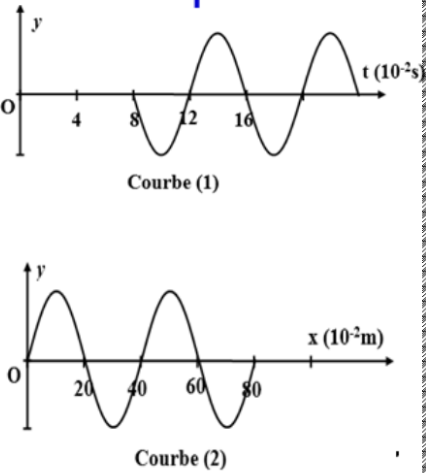
\includegraphics[width=0.32\textwidth]{./img/fig02.png}

  \end{center}
\end{wrapfigure}

 Une lame vibrante en mouvement sinusoïdale de
fréquence N , fixée à l'extrémité S d'une corde élastique $SA$ très longue et tendue
horizontalement, génère le long de celle-ci une onde progressive périodique non
amortie de célérité V. Un dispositif approprié, placé en A, empêche toute
réflexion des ondes. Le mouvement de S débute à l'instant $t = 0$ . Les courbes
(1) et (2) de la figure ci-contre représentent l'élongation d'un point M de la corde,
situé à la distance d de S ,\\et l'aspect de la corde à un instant $t_1$.

\begin{tabular}{c|l}

 0,5 & \makecell[l]{\textbf{1. }Quelle la nature de l’onde propagée le long de la corde? Justifier.}\\
 0,5 & \makecell[l]{\textbf{2. }Identifier, en justifiant, la courbe représentant l'élongation du\\ point M.}\\
 
 2 & \makecell[l]{\textbf{3. }Par exploitation des courbes précédentes, déterminer :\\le retard temporel $\tau$ du point M par rapport à la source S de l'onde
et \\déduire la distance d et l’instant $t_1$ de l’aspect de la corde . }\\

 0,5   & \makecell[l]{\textbf{4. }Représenter $Y_s(t)$ l’élongation du point S}\\

	0,5   & \makecell[l]{\textbf{5. }On donne la relation qui lie la célérité V de l'onde, la tension de la corde et sa masse linéique \\$\mu$ (quotient de la masse sur la longueur) $v = \sqrt{\frac{F}{\mu}}$
	On double la tension de la corde $(F' = 2F)$ sans\\modifier la fréquence N. Montrer que $\lambda' = \sqrt{2}.\lambda$ et calculer sa valeur . }\\

\end{tabular}


\section*{Partie 2 : Étude du phénomène ondulatoire. \dotfill(4pts) }
\begin{wrapfigure}[6]{r}{0.29\textwidth}
  \begin{center}
	  \vspace{-1.5cm}
	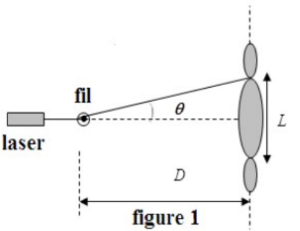
\includegraphics[width=0.23\textwidth]{./img/diff.png}
  \end{center}
\end{wrapfigure}


On réalise une expérience en utilisant un LASER,(figure 1) : la tache lumineuse centrale L conduisent
aux résultats suivants : $a = 0,100mm$ et $D=5,00m$ ; $L=17mm$.

\begin{tabular}{c|l}
	1 & \makecell[l]{\textbf{1. }Quel est le nom du phénomène observé et déduire la nature de \\la lumière  ?}\\
	0,5	&\makecell[l]{\textbf{2. } a l’aide de la figure 1, Etablir la relation entre $\theta$, L et D}\\
		0,5& \makecell[l]{\textbf{3. }En utilisant les résultats des mesures, calculer la valeur de l’angle $\theta$ en rad.}\\

	0,5 &\makecell[l]{\textbf{4. }Donner la relation qui lie les grandeurs $\theta$ (écart angulaire), $\lambda$ (longueur d’onde de la
lumière)\\et a (diamètre du fils). Préciser les unités (dans le système international)}\\
	0,5 &\makecell[l]{\textbf{5. }Calculer la valeur de la longueur d’onde $\lambda$. Est-ce qu’elle appartient au domaine visible?}\\

	1 &\makecell[l]{\textbf{6. }Comment différencier expérimentalement une lumière monochromatique d’une lumière
\\polychromatique
	}\\

\end{tabular}

Pour déterminer la longueur d’onde de l’onde lumineuse $\lambda_0= 583nm$ monochromatique  dans un prisme droite
transparent et homogène d’indice de réfraction n , on envoie cette onde sous un angle d’incidence i sur l’une des
faces du prisme dont l’angle de l’ arrêt $A=30$° , Le rayon sort perpendiculairement à la deuxième face de prisme
(l’angle d’incidence r’ et de réfraction i’ sur la deuxième face sont nulles i’=r’=0) La déviation du rayon sortant
par rapport au rayon incident est D=10° (figure ci-contre )
On donne l’indice de réfraction de l’air $n_{air}=1$ .

\begin{tabular}{c|l}
	2 &\makecell[l]{\textbf{1. }Montrer que l’indice de réfraction de prisme à pour expression :$n = \frac{sin(A + D)}{sin(A)}$, et calculer sa valeur.}\\


	1 &\makecell[l]{\textbf{2. }Que peut-on dire à propos du verre constituant le prisme}\\
	
	1 &\makecell[l]{\textbf{3. }Calculer la longueur d’onde du rayon rouge dans le prisme.}\\
	
	1 &\makecell[l]{\textbf{4. }Qu’observe-t-on si on remplace l’onde monochromatique incidente sur
le prisme par la lumière\\blanche ?Nommer ce phénomène }\\
\end{tabular}


\end{document}
